\chapter{Spatially Random Maps}
\label{background}
As studying the effects of random spatial perturbations
on the dynamics of One Dimensional Maps may yield implications for
understanding the dynamics on higher dimensional maps, we present two
case studies:
\begin{enumerate}
\item the logistic map,
\item the circle map.
\end{enumerate}
The random spatial perturbations in both maps are intended to mimic
the noise used in hydraulic modeling for the porosity and hydraulic
conductivity, which is often assumed to be log-normal with an
exponentially decaying spatial correlation. The following sections
offer background information on the characteristics of both maps, with
and without random spatial perturbations. 
\section{Definitions}
One-dimensional maps, such as the logistic map and the circle map, are
analyzed in a variety of ways, e.g. fixed point iterations,
cobweb diagrams, bifurcation diagrams, etc. This section offers some
basic definitions and explanations of these concepts. One Dimensional Maps are a
subclass of dynamical systems in which time is discrete, rather than
continuous. They take the form
\begin{equation*}
x_{n+1}=f(x_n)
\end{equation*}
These maps demonstrate that even simple dynamical systems are capable
of complex behavior, and as such, are also simple examples of
\textbf{chaos}. Although no universal definition of chaos has been
agreed upon, the following working definition is generally acceptable~\cite{strogatz}:
\begin{singlespace}
\begin{definition}
Chaos is aperiodic long-term behavior in a deterministic
  system that exhibits sensitive dependence on initial conditions.
\end{definition}
\end{singlespace}
\begin{enumerate}
\item \textbf{Aperiodic long-term behavior} is another way of stating
  that there are trajectories within the map that do not limit to
  fixed points or more generally quasiperiodic orbits as $n \to \infty$.
\item \textbf{Deterministic} is used to describe systems in which
  there is no random input or parameter. The observed behavior of the
  system arises from its nonlinearity, not from random noise.
\item \textbf{Sensitive dependence on initial conditions} means that
  trajectories that start in almost the same place ($\epsilon$ apart)
  separate quickly. In other words, the system has a
  positive Lyapunov exponent.
\end{enumerate}

The sequence of iterates ${x_0,x_1,...,x_n}$ in a map is
called an \textbf{orbit}. As $n \to \infty$, orbits may converge on a fixed point, or a
set of fixed points. A \textbf{fixed point} $x^*$ of a function $f$ is an element of the
function's domain that is mapped to itself by the function. The stability of the fixed point $x^*$ is
determined by perturbing the fixed point by $\eta$ to see whether it is
attracted to or repelled from $x^*$. A Taylor series expansion around
the perturbation $x_{n+1} = x^* + \eta_{n+1}$ linearizes the map
\begin{align*}
\begin{split}
x^* &= f(x^*)\\
x_{n+1} &= x^* + \eta_{n+1}\\
x^* + \eta_{n+1} &= f(x^* + \eta_n)\\
&= f(x^*) + f'(x^*)\eta_n + \mathcal{O}(\eta_n^2),\\
\eta_{n+1} &= f'(x^*)\eta_n + \mathcal{O}(\eta_n^2).\\
\end{split}
\end{align*}
Neglecting the higher order terms in $\mathcal{O}(\eta_n^2)$ leaves
$\eta_{n+1} = f'(x^*)\eta_n$. The multiplier is $\hat{\lambda} =
f'(x^*)$. Solutions of the map are found by extending the recursion:
\begin{align*}
\begin{split}
\eta_{1} &= \hat{\lambda}\eta_0\\
\eta_{2} &= \hat{\lambda}\eta_1 = \hat{\lambda}^2\eta_0\\
&...\\
\eta_{n} &=\hat{\lambda}^n\eta_0\\
\end{split}
\end{align*}
If $|\hat{\lambda}| = |f'(x^*)| > 1$, $\lim_{n \to \infty}\hat{\lambda}^n = \infty$, and
the fixed point $x^*$ is \textbf{linearly unstable}. If $|\hat{\lambda}| = |f'(x^*)| < 1$, $\lim_{n \to
  \infty}\hat{\lambda}^n = 0$, and the fixed point $x^*$ is
\textbf{linearly stable}. If
$|\hat{\lambda}| = |f'(x^*)| = 1$ the $\mathcal{O}(\eta_n^2)$ terms
determine the local stability~\cite{strogatz}. Linear stability is
linked to nonlinear stability by the Hartman-Grobman Theorem~\cite{meiss}.
\begin{singlespace}
\begin{theorem}
Hartman-Grobman Theorem: Let $x^*$ be a hyperbolic equilibrium point of a $C^1$
vector field $f(x)$ with flow $\phi_t(x)$. Then there is a
neighborhood $N$ of $x^*$ such that $\phi$ is topologically conjugate to its linearization on $N$.
\end{theorem}
\end{singlespace}
The Hartman-Grobman theorem states the behavior of the linearized
dynamical system near a fixed point is equivalent to the
behavior of the nonlinear system near the same point, as long as the
multiplier $|\hat{\lambda}|\neq 1$. Therefore, the results of linear stability
analysis of fixed points translates to nonlinear stability. 

A \textbf{cobweb diagram} is a graphical representation of the orbit iterations. The method of the cobweb diagram can be outlined in four steps:
\begin{enumerate}
\item Begin at the Cartesian coordinate pair $(x_0, f(x_0))$, which
  may also be written as $(x_0, x_1)$
\item Plot horizontally the distance from $(x_0, f(x_0)=(x_0, x_1)$ to $(f(x_0),
  f(x_0))=(x_1, x_1)$
\item Plot vertically from $(f(x_0), f(x_0))=(x_1, x_1)$ to $(f(x_0), f(f(x_0)))=(x_1, x_2)$
\item Repeat steps 2-3 until convergence or divergence is determined:
  $(x_n, x_{n+1}) \to (x_{n+1}, x_{n+1}) \to (x_{n+1},x_{n+2})$
\end{enumerate}
\begin{figure}[!h]
\caption[Example of a Cobweb Diagram]{A One Dimensional Map (blue) and
  the line $x_{n+1}=x_n$ (red) with a few iterates of the cobweb
  diagram (green). Cobweb diagrams encapsulate the dynamics of the map at a glance.}
    \begin{center}
	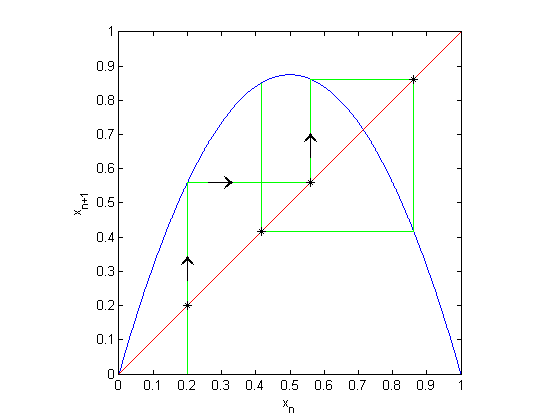
\includegraphics[scale=0.8]{figs/cobweb_ex.png}
    \end{center}
\end{figure}

\textbf{Lyapunov exponents} are a way of classifying a the sensitive
dependence on initial conditions in any given map. They are defined as follows:
\begin{equation}
\lambda(x_0) = \lim_{n \to \infty} \frac{1}{n} \sum_{i=0}^{n-1} \ln |f'(x_i)|
\end{equation}
$\lambda(x_0)$ is the same for all initial conditions $x_0$ in the same \textbf{basin of
attraction}. The basin of attraction for an attracting fixed point
$x^*$ is defined as the set $S=\{x_0:x(t) \to x^*, t \to \infty\}$, i.e.
the set of initial conditions $x_0$ that are drawn to the fixed point
as time goes to infinity~\cite{strogatz}. For stable fixed points and periodic orbits, $\lambda(x_0) < 0$,
and for chaotic attractors, $\lambda(x_0)>0$.

\section{Logistic Map}
\subsection{Deterministic case}
\hspace{5mm}The Logistic map is a quadratic recursive equation that maps the domain
$[0,1] \rightarrow [0,1]$. It is a commonly studied topic in nonlinear dynamics and has
applications in population modeling. Robert May popularized the
logistic map in 1976~\cite{may}. He demonstrated even simple nonlinear
maps could have complicated dynamics. There is one parameter in the
expression, $r$, which can take any value in the range [0,4] so that
[0,1] is an invariant set of the map. $f:[0,1]\to [0,1]$
\begin{equation}\label{logmap}
x_{n+1} = f(x_n) = rx_n(1-x_n)
\end{equation}
We require $[0,1]$ to be invariant in $f$ because of the stipulations
of the fixed point convergence theorem~\cite{atkinson}.
\begin{singlespace}
\begin{theorem}\label{thm:fp}
Let $D$ be a closed, bounded and convex set in the plane. Assume the
components of the iterative map $g(x)$ are continuously differentiable at all points of
$D$, and further assume: 
\begin{enumerate}
\item $g(D) \subset D$
\item $\lambda =\max_{x\in D}||G(x)||_\infty < 1$, where $G(x)$ is the Jacobian of
$g(x)$
\end{enumerate}
Then, 
\begin{itemize}
\item $x=g(x)$ has a unique solution $\alpha \in D$
\item For any initial point $x_0 \in D$, the iteration will converge
  in $D$, i.e. $\lim_{t \to \infty}x_t = \alpha$
\item $||\alpha - x_{n+1}||_\infty \leq
  (||G(\alpha)||_\infty+\epsilon_n)||\alpha - x_n||_\infty$ with
  $\epsilon \to 0$ as $n\to \infty$
\end{itemize}
\end{theorem}
\end{singlespace}
 For a fixed initial condition $x_0$ and $r$, the long term behavior of
the map may be obtained by fixed point iteration, using~(\ref{logmap}). 
\begin{figure}[!h]
\caption[Deterministic logistic map, stable orbit]{Deterministic Logistic Map (blue) for $r=3.2$. There is a stable period
4 orbit. The period is calculated by counting the number
of crossings from the cobweb diagram (green) on the line $x_{n+1}=x_n$
(red). The transient iterations (the first 500) were removed to make
the long-term behavior of the orbit more obvious.}\label{fig:detlogstable}
    \begin{center}
	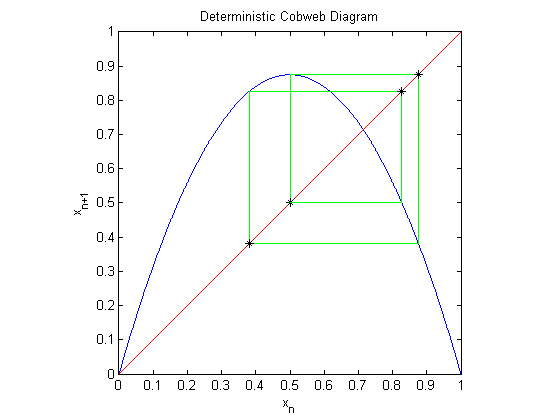
\includegraphics[scale=0.8]{figs/det_cobweb.png}
    \end{center}
\end{figure}
For example, Figure~\ref{fig:detlogstable}
demonstrates a stable period 4 orbit, whereas Figure~\ref{fig:detlogunstable}
demonstrates a possibly chaotic orbit. 
\begin{figure}[!h]
\caption[Deterministic logistic map, unstable orbit]{Deterministic
  Logistic Map (blue) for $r=3.8$. There appears to be no
  stable orbit. The cobweb diagram (green) behaves erratically, even
  after removing the transient behavior. For values of $r \in
  [3.5,4]$, the system is chaotic.}\label{fig:detlogunstable}
	\begin{center}
		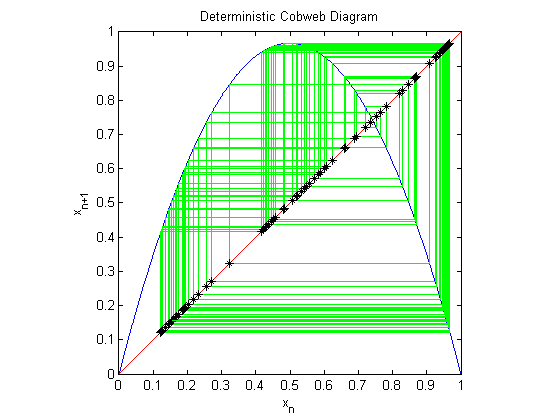
\includegraphics[scale=0.8]{figs/chaos.png}
	\end{center}
\end{figure} 
The effects of the parameter $r$ are
tabulated in Table~\ref{tbl:bif} and also graphically visualized in
Figure~\ref{fig:bif}. 
\begin {table}[!h]
\begin{center}
\caption[Behavior of the deterministic map as $r$ is varied]{As $r$ is
varied over [0,4], the logistic map undergoes notable changes in terms
of stability~\cite{may}.}\label{tbl:bif}
\begin{tabular}{ | p{4cm}| p{8cm}|}   \hline
$r \in [0,1]$ & convergence to the stable Period
1 orbit, $x=0$ \\ \hline
$r \in [1,2]$ & convergence to the stable Period 1
orbit, $x = \frac{r-1}{r}$\\ \hline
$r \in [2,3]$ & convergence to the stable Period 1
orbit, $x = \frac{r-1}{r}$, but at a slower rate\\ \hline
$r \in [3,3.44949]$ & emergence of stable Period 2 orbits\\ \hline
$r \in (3.44949, 3.54409)$ & emergence of stable Period 4 orbits\\ \hline
$r \in [3.54409,3.56995)$ & period doubling cascade\\ \hline
$ r \approx 3.56995 $ & onset of chaos\\\hline
$r \in (3.56995,4]$ & mostly chaotic behavior, but there are islands of
stability (eg. Period 3 orbits for $r \approx 3.82843$) \\\hline
\end{tabular}
\end{center}
\end {table}
Most notably, there is no chaos for values of $r
< 3.5$, and for $r > 3.5$, the system is mostly chaotic, although
there are islands of stability interspersed throughout the \textbf{bifurcation
diagram}. A bifurcation is a qualitative change in dynamics, such as
the creation or destruction of fixed points, or a change in their
stability~\cite{strogatz}. These changes are strongly dependent on the
parameters of the system. Therefore, a bifurcation diagram is a
visual demonstration of the change in dynamics of a system as its
parameters are varied. 
\begin{figure}[!h]
\caption[Bifurcation diagram for the deterministic logistic map]{The behavior in Table~\ref{tbl:bif} may be graphically represented
in a bifurcation diagram. The horizontal axis shows the value of $r$ as it ranges over
  $[0,4]$. The vertical axis plots the long term behavior of iterates
  in the deterministic logistic map. The left diagram ranges from $r\in
  [0,4]$, and the right diagram ranges from $r\in [2.5,4]$. Notice the
  islands of stability in the chaotic region of the map.}\label{fig:bif}
\centering
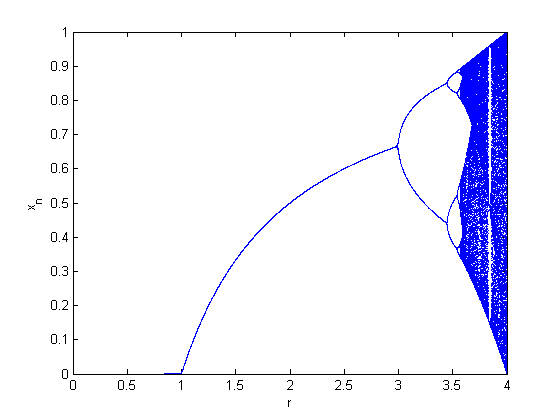
\includegraphics[width=.5\textwidth]{figs/det_bif_1.png}\hfill
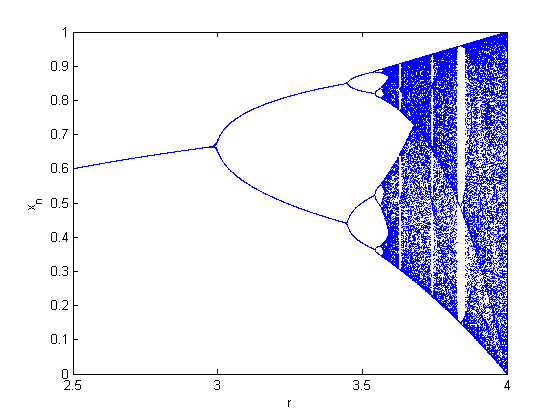
\includegraphics[width=.5\textwidth]{figs/det_bif_2.png}
\end{figure}
Bifurcation diagrams are constructed by
plotting the long term behavior of the map as a function of its
parameters. In the case of~(\ref{logmap}), we plot the
locations of the stable orbits as $r$ is varied over $[0,4]$.

\subsection{Random case}
The spatially random logistic map replaces the parameter $r$ from~(\ref{logmap}) with a random function of space, $R:[0,1]\to [0,4]$. As before,
$f:[0,1]\to [0,1]$.
\begin{equation}\label{randlogmap}
x_{n+1} = f(x_n) = R(x_n)x_n(1-x_n)
\end{equation}
The noise in hydraulic modeling is often assumed to be log-normal with an
exponentially decaying spatial correlation. Thus, we let
\begin{equation}\label{R}
\xi(x)=\ln(R(x)) 
\end{equation}
be a random variable with mean $E[\xi(x)] = \ln(r)$, variance
Var$(\xi(x))=E[(\xi(x) - \ln(r))^2]=E[\xi(x)^2]-(\ln(r))^2$, and
covariance (assuming homogeneity, so $C(x)$ is independent of $y$)
\begin{align}
\begin{split}\label{cor}
C(x) &=E[(\xi(x+y) - E[\xi(x)])(\xi(y)-E[\xi(x)])] \\
&= E[(\xi(x+y) -\ln(r))(\xi(y)-\ln(r))] \\
\end{split}
\end{align}
$C(x)$ is also called a correlation function, which
describes how variables at different positions in space are
related. Correlations are strongest when iterates are nearby, and
correlations typically gradually decay as
the distance between two iterates increases, although random processes
could violate this assumption. 
Figure~\ref{fig:rlogstable} demonstrates one realization of the
spatially random logistic map.
\begin{figure}[!h]
\caption[Random logistic map, stable orbit]{One instance of a random
  logistic map (blue), which was iterated for 1000 steps. The map has converged to a stable period 4 orbit (green). Notice the
  ``wiggliness'' in the parabola shape. $r=3.5,L=0.05,N=200,\sigma=0.0061$}\label{fig:rlogstable}
	\begin{center}
		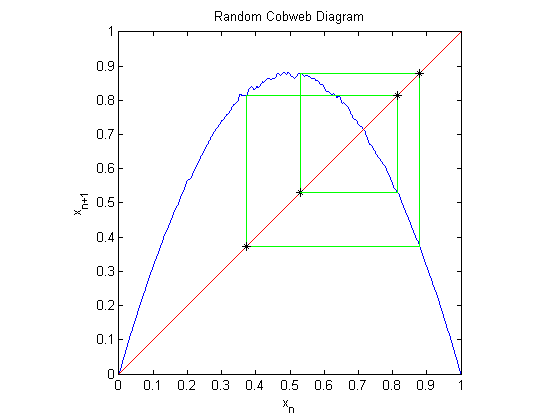
\includegraphics[scale=0.7]{figs/rand_cobweb.png}
	\end{center}
\end{figure}
We can construct such a
function $\xi(x)$ on $[0,1]$ that satisfies the above requirements with a Fourier
Series.
\begin{align}\label{fs1}
\begin{split}
\xi(x) &= \ln(r) + \sum_{n \in \mathbb{Z}}\hat{\xi_n}e^{2\pi inx}\\
\hat{\xi_n} &= a_n + ib_n = \hat{\xi}_{-n}^*
\end{split}
\end{align}
where the $*$ operator denotes the complex
conjugate. $\hat{\xi_{-n}},\hat{\xi^*}_{n} \in \mathbb{C}$ are
independent random variables. We can combine
the equations in~(\ref{fs1}) to arrive at the following form for
$\xi(x)$.
\begin{align}\label{fs2}
\xi(x) = \ln(r) + 2\sum^N_{n=1}a_n\cos(2\pi nx)-b_n\sin(2\pi nx)
\end{align}
where $N$ represents the number of Fourier modes in the sum, and is an
upper limit (necessary for numerical
simulations) that we impose on the summation.\footnote{In practice, $N
  \approx 10/L$, where $L$ represents the correlation length. $N$
  should be chosen to be large enough such that the Fourier amplitudes
may decay as more terms are included. This restriction will ensure the
fluctuations are log-normal.} (\ref{fs2}) assumes
$a_0=b_0=0$ for symmetry, but $\hat{\xi_0}$ may be a random variable as well. We can impose more restrictions of $\hat{\xi}_n$; in particular,
we require the real and imaginary parts $(a_n,b_n)$ of $\hat{\xi}_n$
to be independent with mean $\mu$ and variance $\sigma^2$
\begin{align}
\begin{split}\label{Sn}
\mu&=E[\hat{\xi}_n]=0\\
\sigma^2&=E[\hat{\xi}_n^2]-(E[\hat{\xi}_n])^2=E[\hat{\xi}_n^2]\\
S_n&=\sigma^2\\
\end{split}
\end{align}
where $S_n$ is the spectral density of the log-fluctuations. This
implies
\begin{align*}
\begin{split}
E[\hat{\xi}_n\hat{\xi}_m]&=E[|\hat{\xi}_n||\hat{\xi}_n|\delta_{m+n}]\\
&=\delta_{m+n}E[|\hat{\xi}_n|^2]\\
&=\delta_{m+n}S_n\\
\end{split}
\end{align*}
\begin{displaymath}
   E[\hat{\xi}_n\hat{\xi}_m] = \left\{
     \begin{array}{lr}
       \delta_{m+n}S_n & : m = -n\\
       0 & : m \neq -n\\
     \end{array}
   \right.
\end{displaymath} 
The spectral density $S_n$ is defined as the Fourier transform of the
correlation function~(\ref{cor}).
\begin{align*}
\begin{split}
\hat{C}_k &= \int_{0}^{1}C(x)e^{-2\pi ikx}dx\\
&= \sum_{m,n} \int_{0}^{1} E[\hat{\xi}_n\hat{\xi}_m] e^{2\pi
  im(x+y)}e^{2\pi iny}e^{-2\pi ikx}dx\\
&=S_k
\end{split}
\end{align*}
A simple spectrum that falls off quickly is
\begin{align}\label{spec}
S_n=\alpha_n e^{-L|n|}
\end{align}
where $L \in [0,1]$ is the correlation length (and is fixed
for each simulation). This choice of $S_n$ corresponds to a correlation function
\begin{align}
\begin{split}
C(x) &= \sum_{n\in \mathbb{Z}}S_ne^{2\pi inx}=\sum_{n\in \mathbb{Z}}\alpha \frac{1}{e^{L|n|}}e^{2\pi inx}\\
&= \alpha + \sum_{n=1}^{\infty}\alpha e^{2\pi
  inx-L|n|}+\sum_{n=-1}^{-\infty}\alpha e^{-2\pi inx-L|n|}\\
&= \alpha+\alpha \sum_{n=1}^{\infty}(e^{2\pi ix-L})^n+\alpha \sum_{m=1}^{\infty}(e^{-2\pi ix-L})^m\\
&=\alpha + \alpha \frac{e^{2\pi ix-L}}{1-e^{2\pi ix-L}} +\alpha
\frac{e^{-2\pi ix-L}}{1-e^{-2\pi ix-L}}\\
&=\alpha \left(1+ \frac{-2e^{-2L}+2\cos(2\pi x)e^{-L}}{e^{-2L}-2\cos(2\pi x)e^{-L}+1} \right)\\
\end{split}
\end{align}
Finally,
\begin{align}\label{cx}
C(x)= \alpha \frac{e^{2L}-1}{e^{2L}-2\cos(2\pi x)e^L+1}
\end{align}
Above, the parameter $\alpha$ is a constant used to normalize $C(x)$. To normalize $C(x)$,
let $C(0)=\sigma^2$. In other words, at position $x=0$, the
correlation function is equal to the variance from~(\ref{Sn}).
\begin{align}
\begin{split}\label{a}
\sigma^2&= \alpha \frac{e^{2L}-1}{e^{2L}-2\cos(0)e^L+1}\\
\alpha &=\sigma^2 \frac{e^{2L}-2e^{L} +1}{e^{2L}-1}\\
\alpha &=\sigma^2
\frac{(e^{L}-1)^2}{(e^{L}-1)(e^{L}+1)}\\
\alpha &= \sigma^2 \tanh(L/2)
\end{split}
\end{align}
Such a function $C(x)$ is demonstrated in Figure~\ref{fig:correlation}
for various values of $L$.
\begin{figure}[htp]
\caption[The correlation function $C(x)$]{The correlation function
  $C(x)$ for $L \in \{0.1,0.5,1\}$. For small $L$
  (leftmost graph), the correlation is stronger between iterates than for large $L$
  (rightmost graph).}\label{fig:correlation}
\centering
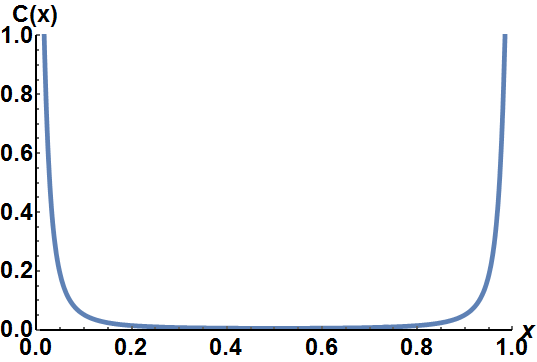
\includegraphics[width=.3\textwidth]{figs/correlation_L01.png}\hfill
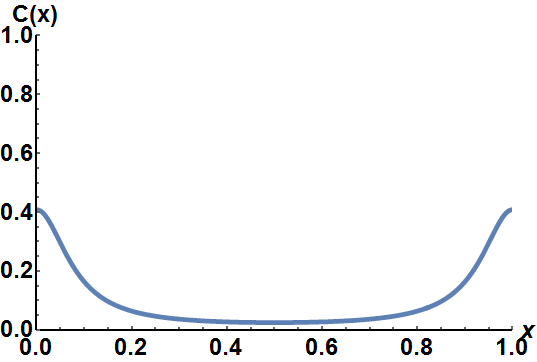
\includegraphics[width=.3\textwidth]{figs/correlation_L05.png}\hfill
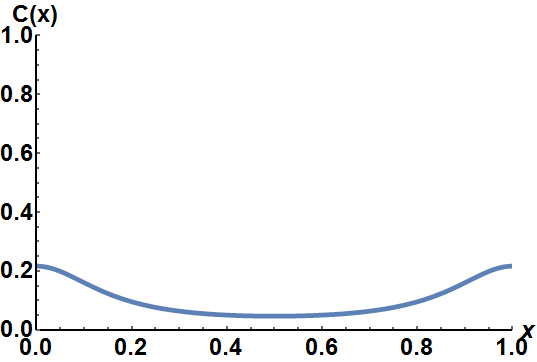
\includegraphics[width=.3\textwidth]{figs/correlation_L1.png}
\end{figure}

Recall Theorem~\ref{thm:fp} stipulates if $x \in D$, then $f(D) \subset
D$ in order for a fixed point to exist. Furthermore, for $[0,1]$ to be an invariant set of $f$, $R(x)$
must be bounded within $[0,4]$, as specified in~(\ref{logmap}). Without enforcing this condition
on~(\ref{Sn}), iterates on~(\ref{randlogmap}) would leave $[0,1]$. One way to accomplish this is to bound
the distribution of $\hat{\xi}_n$ from~(\ref{fs1}). Suppose the probability density
function for $\hat{\xi}_n$ is nonzero only in the complex square centered at the
origin with side length $2M_n$. Thus, $|\hat{\xi}_n| \leq
\sqrt{2}M_n$, and for a fixed $r$, we
can bound $\ln(R(x))$ using~(\ref{R}) and~(\ref{fs1})
\begin{align}
\begin{split}\label{bdnr}
|\ln(R)-\ln(r)|&\leq |\max_{R\in [0,4]}\ln(R) - \ln(r)|=\ln(4/r)\\
|\ln(R)-\ln(r)|&\leq \sum_{n\in \mathbb{Z}}|\hat{\xi}_n| \\
&\leq \sqrt{2}M_0+2\sum_{n=1}^\infty \sqrt{2}M_n\\
&\leq \ln(4/r)
\end{split}
\end{align}
The sequence of side lengths $M_n$ must be summable. 
\begin{figure}[!h]
\caption[Uniform Distribution over a Square Region]{The probability
  density function of $\hat{\xi_n}$ is uniformly distributed across
  this square region, centered at the origin. The square region has
  side length $2M_n$ and area $4M_n^2$.}\label{fig:square}
	\begin{center}
		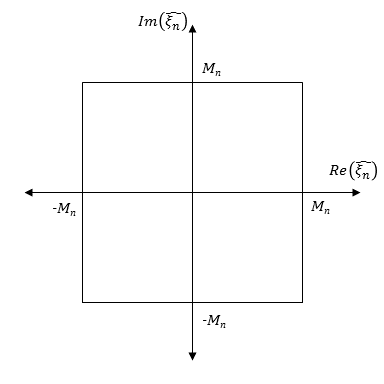
\includegraphics[scale=0.7]{figs/square.png}
	\end{center}
\end{figure}
Suppose $\hat{\xi}_n$ is uniformly distributed, so 
\begin{displaymath}\label{eq:square}
   h(\hat{\xi}_n) =h(a,b)= \left\{
     \begin{array}{lr}
       \frac{1}{4 M_n^2} & |\hat{\xi}_n| \leq \sqrt{2}M_n\\
       0 & |\hat{\xi}_n| > \sqrt{2}M_n\\
     \end{array}
   \right.
\end{displaymath} 
where $h:\mathbb{C}\to [0,1]\in \mathbb{R}$ is the probability density
function of $\hat{\xi}_n$. To find the relationship between $S_n$ and
$M_n$, recall that $S_n$ is defined as the variance of the
log-fluctuations~(\ref{Sn}). Thus, 
\begin{align}
\begin{split}\label{Mn}
S_n&=E[|\hat{\xi}_n|^2] = E[a^2+b^2]\\
 &= \frac{1}{4M_n^2}\int_{-M_n}^{M_n}\int_{-M_n}^{M_n}a^2+b^2\,da\,db\\
&=\frac{2}{3}M_n^2\\
M_n&=\sqrt{\frac{3}{2}S_n}
\end{split}
\end{align}
Finally, using the expression for $\alpha$~(\ref{a}), the
expression for $M_n$~(\ref{Mn}), and the sum from~(\ref{bdnr}), let
\begin{align*}
A = \sqrt{2}M_0+2\sum_{n=1}^\infty \sqrt{2}M_n \leq \ln(4/r)
\end{align*}
Then, we find
\begin{align*}
\begin{split}
A &=\sqrt{2}\left(\sqrt{\frac{3}{2}\alpha} +
2\sqrt{\frac{3}{2}\alpha}\sum_{n=1}^{\infty}e^{-Ln/2}\right) \\
&= \sqrt{3}\alpha\left(1+ \frac{2e^{-L/2}}{1-e^{-L/2}} \right)\\
&= \sqrt{3}\sigma
\sqrt{\tanh(L/2)}\left(\frac{e^{L/2}+1}{e^{L/2}-1} \right)\\
&= \sqrt{3}\sigma \frac{\sqrt{\tanh(L/2)}}{\tanh(L/4)} \leq \ln(4/r).\\
\end{split}
\end{align*}
Thus, the standard deviation $\sigma$ must be bounded from below by
zero and from above by
\begin{align}\label{sigma}
0<\sigma<\ln(4/r)\frac{1}{\sqrt{3}}\frac{\tanh(L/4)}{\sqrt{\tanh(L/2)}}.
\end{align}
Figure~\ref{fig:R} is a sample realization of a function $R(x)$ that
behaves according to~(\ref{sigma}).
\begin{figure}[!h]
\caption[The function $R(x)$]{The function $R:[0,1]\to [0,4]$ where
  $\sigma=0.0386, L=0.1, r=3.5, N=100$}\label{fig:R}
	\begin{center}
		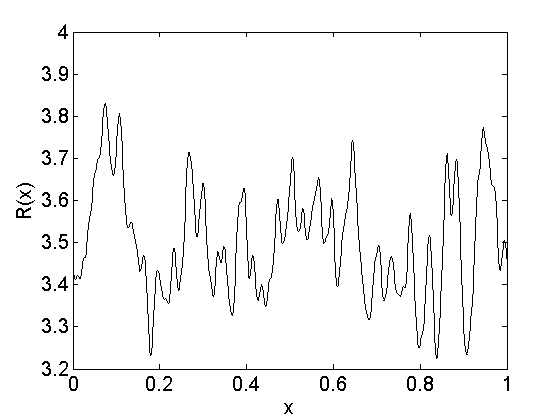
\includegraphics[scale=0.65]{figs/xi.png}
	\end{center}
\end{figure}

In summary, for each realization of the random logistic map,
we have uniform random variables $a_n,b_n \sim Unif(-M_n,M_n)$ that correspond to the
Fourier modes $n$ of $\xi(x)$ from~(\ref{fs2}) whose bounds are set by
$M_n= \sqrt{\frac{3}{2}S_n}$, where $S_n=\alpha e^{-L|n|}$, the
spectral density, was chosen to decay exponentially fast. $\alpha = \sigma^2 \tanh(L/2)$ is a normalization constant for the corresponding
correlation function $C(x)$, where the standard deviation $\sigma$
must be bound according to~(\ref{sigma}) in order to restrict $R(x)$
to $[0,4]$ to ensure $[0,1]$ is an invariant set of
$f$. Figure~\ref{fig:envelope} depicts rough estimates\footnote{The
  maxima and minima over 500 samples were recorded and plotted in
  these figures.} of upper and lower bounds for the random logistic
map for various sets of parameters. 
\begin{figure}[htp]
\caption[Upper and lower bounds on the random logistic map]{A coarse
  demonstration (500 samples) of the upper and lower bounds of the random logistic
  map. Sample realizations are shown in red. From left to right:
  $\{\sigma=0.0773,r=2.7,L=0.9,N=112\}, \{\sigma=0.0061,r=3.5,L=0.05,N=200\},\{\sigma=0.0050,r=3.7,L=0.1,N=100\}$
  }\label{fig:envelope}
\centering
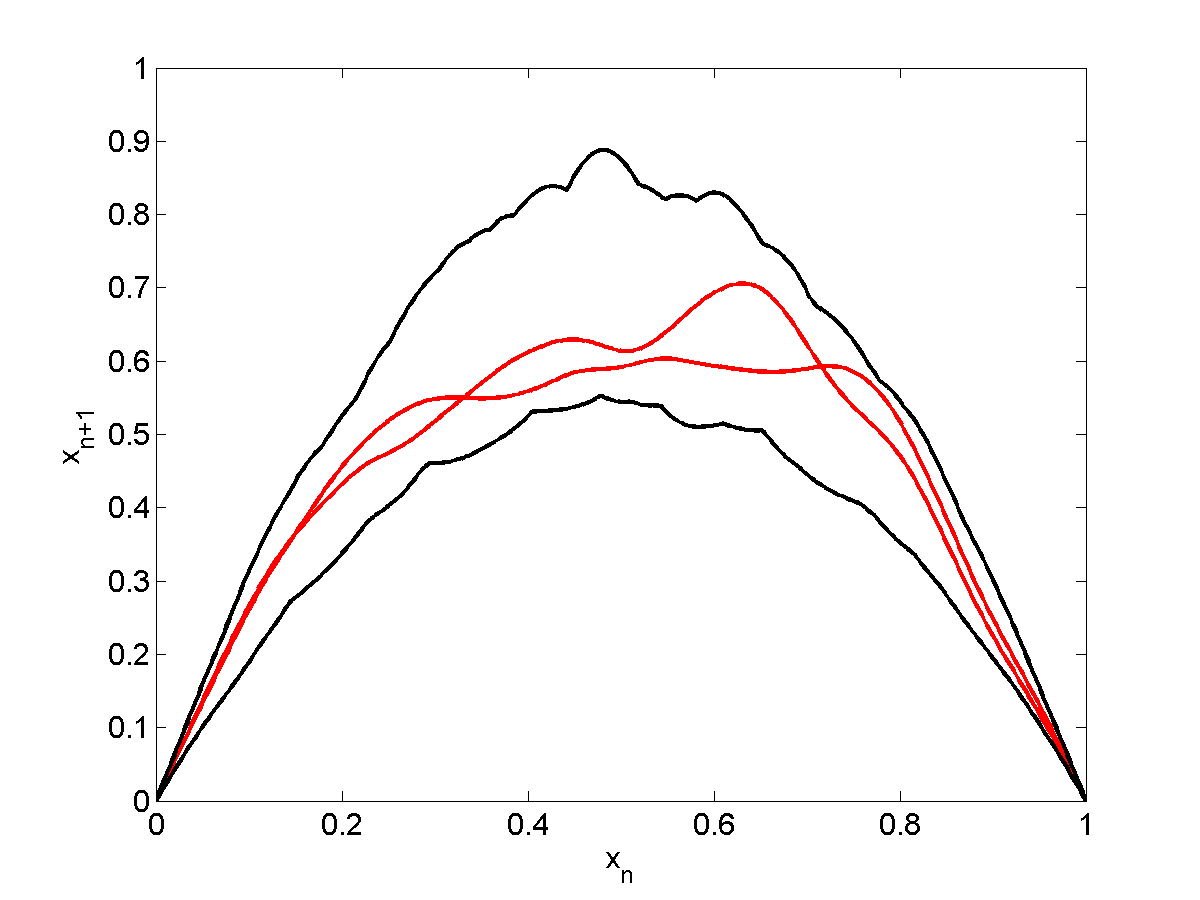
\includegraphics[width=.3\textwidth]{figs/envelope_500_r27_L09.png}\hfill
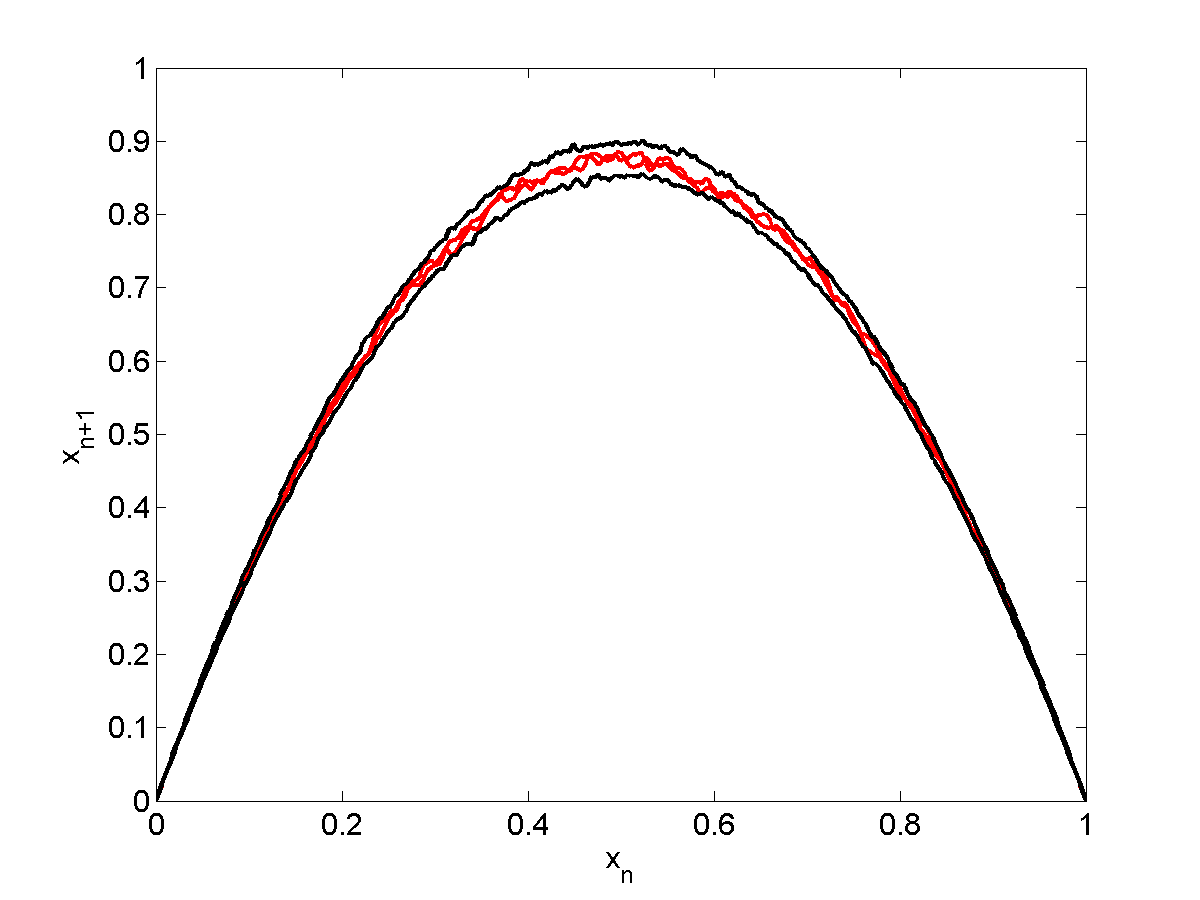
\includegraphics[width=.3\textwidth]{figs/envelope_500_r35_L005.png}\hfill
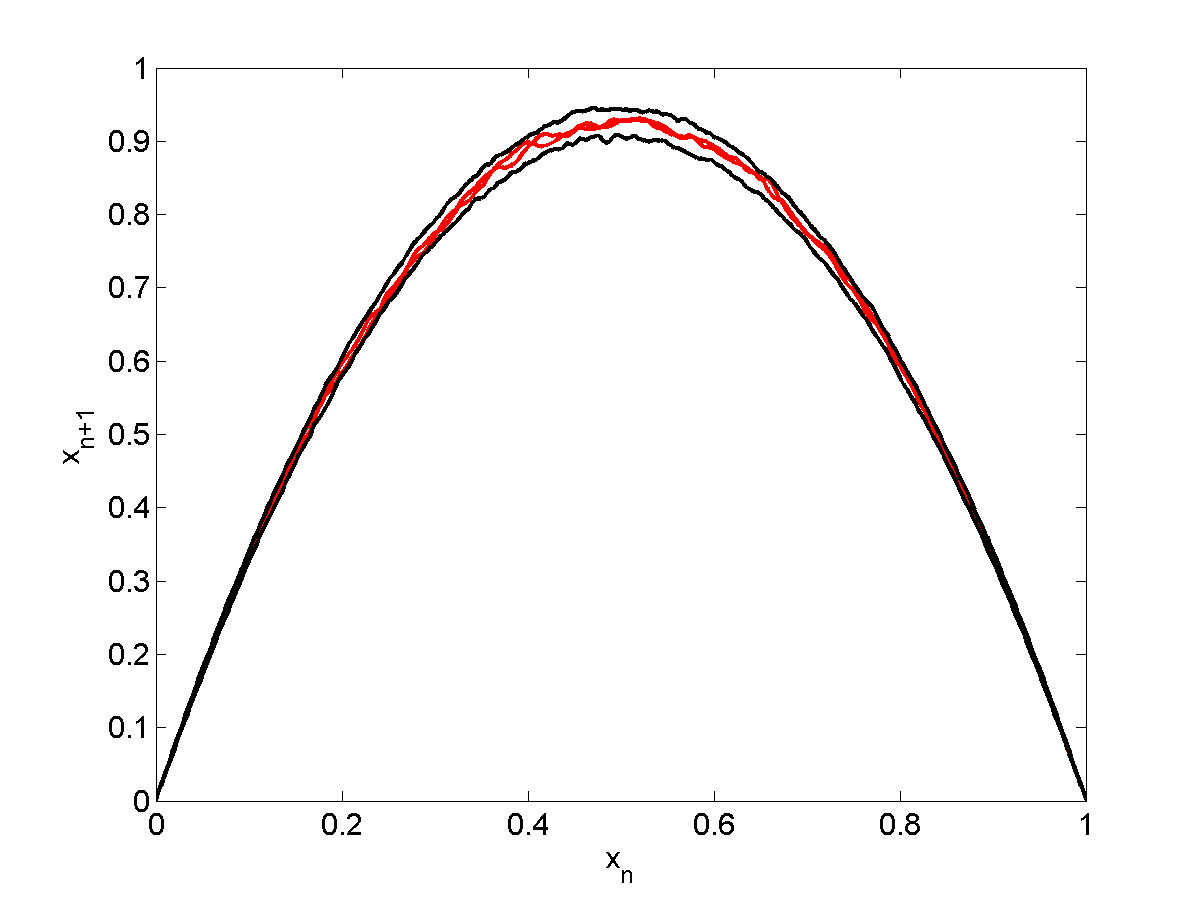
\includegraphics[width=.3\textwidth]{figs/envelope_500_r37_L01.png}
\end{figure}

\section{Circle Map}
The circle map is another
recursive expression whose deceivingly simple form gives way to complicated behavior. It was used to
understand the dynamics of a kicked rotor by Vladimir
Arnold, who is credited for discovery of what are now called the Arnold Tongues, which are
regions of stable periodic motion in the bifurcation diagram of the
map. Generally, a degree-one circle map takes the form
\begin{align*}
x_{n+1}&=f(x)=x_n + \omega + g(x_n) \mod 1\\
g(x_n)&=g(x_n + 1)
\end{align*}
where the angle $x$ has been normalized so that its range is $[0,1)$
instead of $[0,2\pi )$, $\omega$ is the driving frequency of the map, and
$g(x)$ is the nonlinear component of the recursion~\cite{rasband}. The
parameter $\omega$ represents the frequency of the driving
force, which is the external force applied to the
rotor. We define the circle $S^1$ as $\mathbb{R} \setminus \mathbb{Z}$
to avoid factors of $2\pi$.

A phenomenon of \textbf{mode-locking} may occur in the map,
where after $q$ iterations, the new angle differs from the initial
value of $x$ by exactly $p \in \mathbb{Z}$
\begin{align*}
x_{n+q}=x_n+p
\end{align*}
Notice the modulo operator is no longer applied to the map. Thus, this
is the lift of the map from $S^1$ to $\mathbb{R}$. The
rotation number of the orbit is defined by
\begin{align}\label{rho}
\begin{split}
\rho &= \lim_{n \to \infty} \frac{f^n(x)-x}{n}\\
&= \frac{p}{q}
\end{split}
\end{align}
When $\rho \in \mathbb{Q}$, the system is mode-locked, and if $\rho$
does not exist, then the system may be in a chaotic
state. When $\rho \in \mathbb{R} \setminus \mathbb{Q}$, the orbit is quasiperiodic.  

\subsection{Deterministic case}
Arnold introduces the example
\begin{align}\label{detcirc}
x_{n+1}= f(x_n) =  x_n + \omega - \frac{k}{2\pi}\sin(2\pi x_n),
\end{align}
which we will explore as well. There are two parameters: $k \in [0,1]$
is the coupling strength and $\omega \in [0,1]$ is the driving
frequency. To ensure $\forall x \in S^1, f(S^1) \subset S^1$ in~(\ref{detcirc}), we apply the
modulo operator 
\begin{align*}
x_{n+1}=x_{n+1} \mod 1
\end{align*}
to all iterates. The coupling strength $k$
controls the amplitude of the oscillations in the circle map; no
coupling is $k=0$, and the coupling increases as $k \to \infty$. In contrast, $\omega$
applies a positive vertical shift to the map, which causes it to wrap around itself, due to the effects of the modulo operator. The changes in the rotation number $\rho$ as $\omega$ is
varied over [0,1] is graphically demonstrated as a Devil's Staircase
in Figure~\ref{fig:devil_det}. 
\begin{figure}[!h]
\caption[The Devil's Staircase for the deterministic circle map]{The
  plot of $\omega$ vs the rotation number $\rho$ for $k=1$ results in a Devil's
  Staircase, which maps $[0,1]\to [0,1]$. Since the circle map is monotone, $\rho$ is independent of
  the initial value $x_0$. At each $\omega$, $\rho$ is either
  irrational or rational (due to the quasiperiodic cases), which results in a monotonically increasing
  "staircase." The largest steps (where $\rho$ appears constant)
  correspond with the simplest rationals.}\label{fig:devil_det}
	\begin{center}
		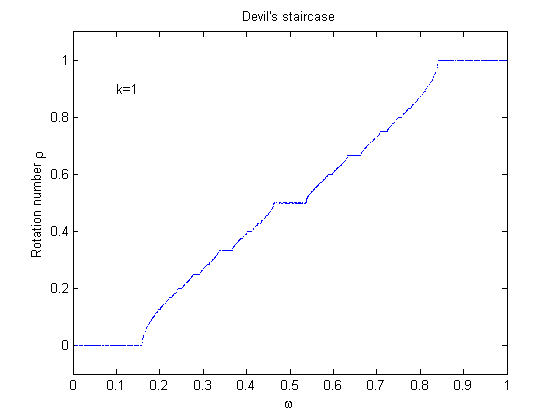
\includegraphics[scale=0.7]{figs/devil_nonrandom_k1.png}
	\end{center}
\end{figure}
The width of each "step" corresponds to the
width of the Arnold Tongues in the bifurcation diagram for $k$ and
$\omega$ in~(\ref{detcirc}). A stable period 2 orbit is shown in
Figure~\ref{fig:dcircstable} for the deterministic circle map, and
Figure~\ref{fig:rcircunstable} shows a diverging orbit.
\begin{figure}[!h]
\caption[Deterministic circle map, stable orbit]{The cobweb
  diagram (green) for a deterministic circle map (blue) with $\omega =
  0.5$ and $k=1$. The line $x_{n+1}=x_n$ is drawn in red. The map
  has converged on a stable period 2 orbit. Transient iterations were removed.}\label{fig:dcircstable}
	\begin{center}
		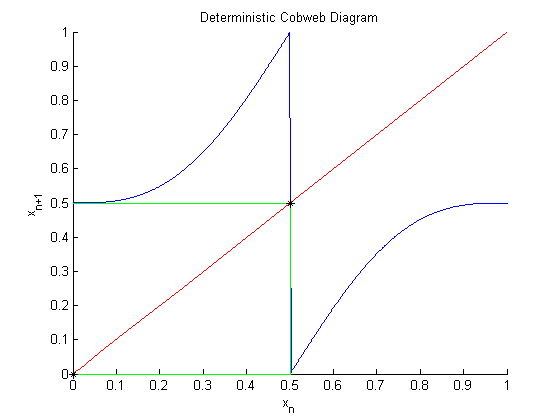
\includegraphics[scale=0.7]{figs/detcirc_cobweb_2.png}
	\end{center}
\end{figure}
\begin{figure}[!h]
\caption[Deterministic circle map, unstable orbit]{The cobweb
  diagram (green) for a deterministic circle map (blue) with $\omega =
  0.6$ and $k=1$. The line $x_{n+1}=x_n$ is drawn in red. The map
  has diverged. Transient iterations were removed.}\label{fig:rcircunstable}
	\begin{center}
		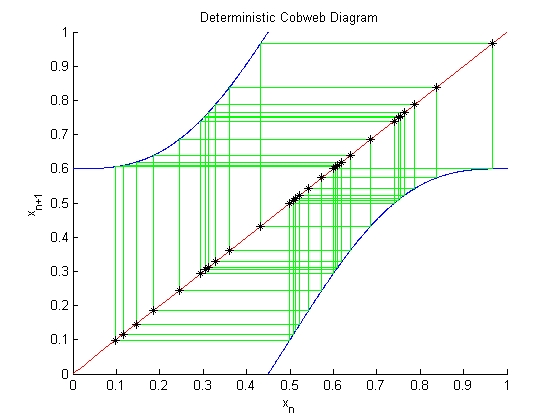
\includegraphics[scale=0.7]{figs/detcirc_cobweb_chaos.png}
	\end{center}
\end{figure}

\subsection{Random case}
We will investigate a spatially random circle map of the form
\begin{align}\label{randcirc}
x_{n+1}= f(x_n) =  x_n + \Omega(x_n) - \frac{k}{2\pi}\sin(2\pi x_n),
\end{align}
where $\omega$ from~(\ref{detcirc}) has been replaced with a function
of space, $\Omega:S^1\to S^1$. Just as in the randomized logistic
map~(\ref{R}), we wish to mimic the noise in hydraulic modeling, so we
will assume that
\begin{align}\label{Omega}
\xi(x) = \ln(\Omega(x)),
\end{align}
where properties of the random variable $\xi(x)$ will be similar to
those of the random logistic map. As before, we apply the definitions $E[\xi(x)] =
\ln(\omega)$, variance Var$(\xi(x))=E[(\xi(x) -
\ln(\omega))^2]=E[\xi(x)^2]-(\ln(\omega))^2$, and covariance
\begin{align}
\begin{split}\label{cor_circ}
C(x) &=E[(\xi(x+y) - E[\xi(x)])(\xi(y)-E[\xi(x)])] \\
&= E[(\xi(x+y) -\ln(\omega))(\xi(y)-\ln(\omega))] \\
\end{split}
\end{align}
A function $\xi(x)$ that satisfies the above requirements may be
constructed with a Fourier Series:
\begin{align}\label{fs_circ}
\begin{split}
\xi(x) &= \ln(\omega) + \sum_{n \in \mathbb{Z}}\hat{\xi_n}e^{2\pi inx}\\
&= \ln(\omega) + 2\sum^N_{n=1}a_n\cos(2\pi nx)-b_n\sin(2\pi nx)\\
\end{split}
\end{align}
As before, $\hat{\xi_n} = a_n + ib_n = \hat{\xi}_{-n}^*$, and the $*$
operator denotes the complex conjugate. The real and imaginary parts
$(a_n,b_n)$ of $\hat{\xi}_n$ are independent with mean
$\mu_n=E[\hat{\xi}_n]=0$ and variance $\sigma_n^2=E[\hat{\xi}_n^2]=S_n$,
where $S_n$ is the spectral density~(\ref{Sn}). The
spectral density decays exponentially, so $S_n$ in this case
takes the same form as for the random logistic map~(\ref{spec}):
\begin{align*}
S_n=\alpha e^{-L|n|}
\end{align*}
However, since we do not require $\Omega(x)$ to be bounded as strictly
as $R(x)$, $\alpha$ may be chosen to be any arbitrary
value\footnote{In the case of the numerical simulations, $\alpha
  \approx 10^{-5}$}. We use the same uniform probability density
function $h:\mathbb{C}\to [0,1]\in \mathbb{R}$ in~(\ref{eq:square})
and Figure~\ref{fig:square}. In Figure~\ref{fig:rcircstable}, a realization of the
random circle map is shown, where the orbit converges to a period 4 orbit.

Overall, we have a much simpler set of equations for the circle map
than for the logistic map since $\Omega(x)$ is unrestricted. For each realization of the map, we choose
a set of random variables, $a_n, b_n \sim Unif(-M_n,M_n)$, that
correspond to the Fourier modes of $\xi(x)$. Their magnitudes decrease
as $M_n=\sqrt{\frac{3}{2}S_n}$ diminishes exponentially, due to the
exponential term in $S_n=\alpha e^{-L|n|}$, where $\alpha$ is an arbitrary
constant. 
\begin{figure}[!h]
\caption[Random circle map, stable orbit]{The cobweb
  diagram (green) for a random realization of the circle map (blue) with $\omega =
  0.3$ and $k=1$. The line $x_{n+1}=x_n$ is drawn in red. The orbit
  has converged to a stable period 4 orbit. Its basin of attraction is
  $S^1$. Transient iterations were removed.}\label{fig:rcircstable}
	\begin{center}
		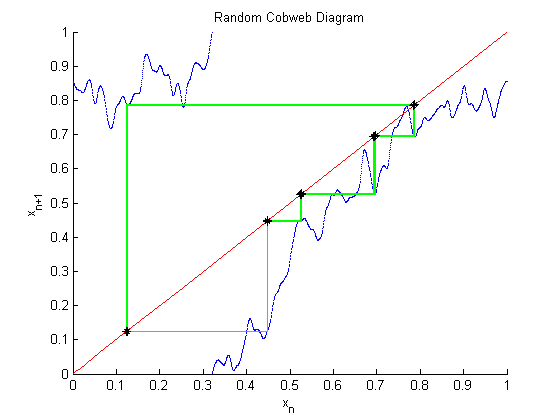
\includegraphics[scale=0.7]{figs/randcirc_cobweb.png}
	\end{center}
\end{figure}

% \singlespacing	% <------------------------------

% This paragraph was preceded by the
% command \verb2\singlespacing2.
% See the Specifications of the Grad School for instructions
% about when single spacing is appropriate in a thesis.

% \doublespacing	% <------------------------------

% And now, here is an example of using the macros
% \verb2\begin{singlespace}2 and \verb2\end{singlespace}2;
% another way to get single-spacing.

% \begin{singlespace}	% <-----------------------------
% Two cases are studied in the present work which differ only in the
% boundary conditions.  Each different boundary condition model a
% different source of instability.  The boundary of the first case
% consists of a steady, axisymmetric sidewall radial velocity boundary
% and a time-dependent, non-axisymmetric endwall axial velocity
% boundary.  The second case is studied with a fixed impermeable axial
% velocity along the endwall and a combination axisymmetric steady and
% non-axisymmetric unsteady radial velocity along the sidewall.
% \end{singlespace}	% <-----------------------------


% Usually you want to use a table produced by some other
% software, such as Excel, rather than try to do it using
% \LaTeX macros.  If the table is saved/printed to a PDF file,
% then it can be displayed using the
% $\backslash${\tt includegraphics} macro
% inside a {\tt table} environment:


% \begin{table}
%     \caption[Table from a PDF file]{
% 	This table wasn't constructed with \LaTeX{}
% 	commands, but resides in PDF file
% 	({\tt tableD.pdf})
% 	created by some other software.
% 	}
%     \begin{center}
% 	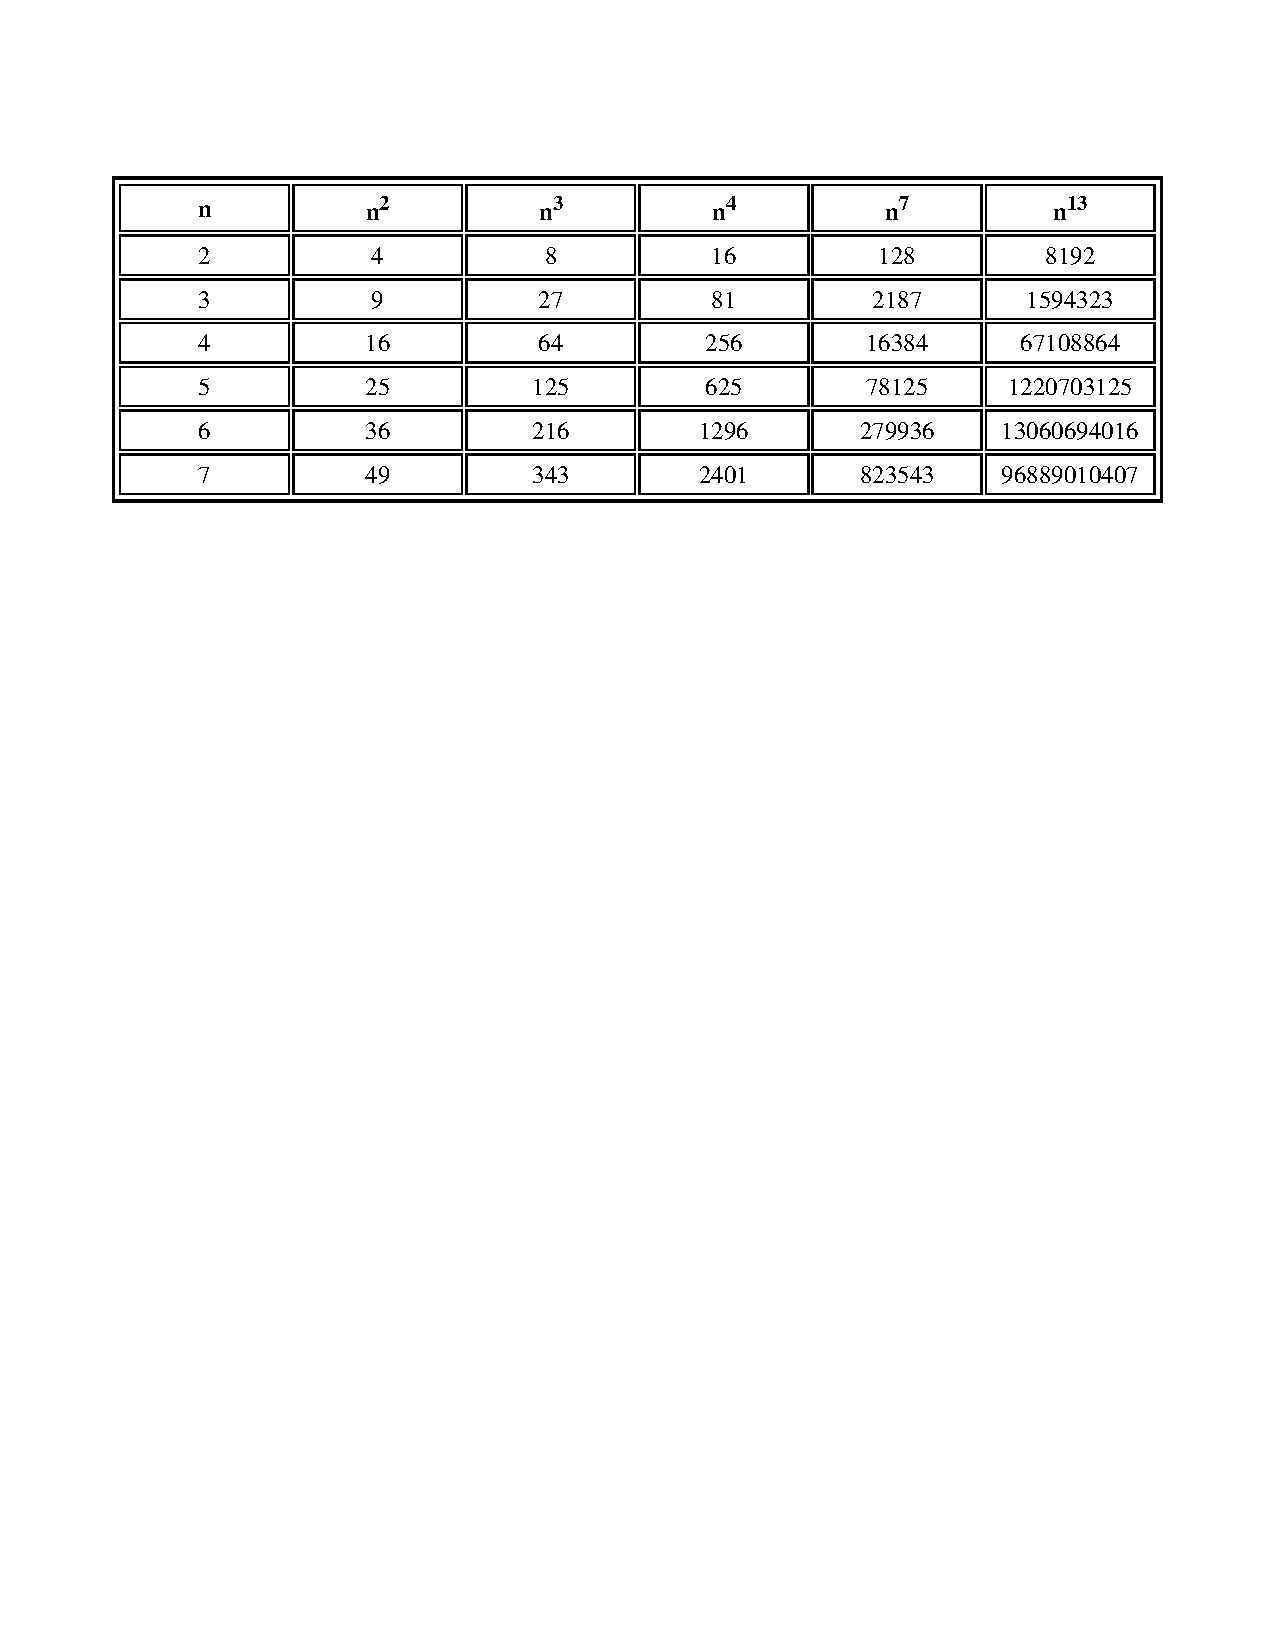
\includegraphics[width=5.45in]{figs/tableD.pdf}
%     \end{center}
% \label{pdftable}
% \end{table}


% Some of the boundary conditions are:

% \begin{eqnarray}
%   z=0; && V_z = \twochoices
% 	{0, && t\leq0}
% 	{\widetilde{F}_{zw}(r,\theta,t), && t>0}
% 						\label{eq:endwall} \\
%   z=0; && V_{\theta}=V_r=0			\label{eq:endnoslip} \\
%   r=0; && P,\rho,T,V_r,\vth,V_z~\mbox{finite},	\label{eq:centerline} \\
%   r=1; && V_r= F_{rws}(z),			\label{eq:injection} \\
%   r=1; && V_z=\vth =0,				\label{eq:sidenoslip}
% \end{eqnarray}
% and solutions must be periodic in $\theta$.

% If you don't believe this stuff, check out
% Mulick\cite{mulick} and Baylor\cite{baylor}.


